\documentclass[20pt]{report}
\usepackage{amsmath, amssymb,amsmath}

\usepackage[spanish, es-lcroman]{babel}  
\usepackage[spanish]{babel}
\usepackage{multicol}
\usepackage{graphicx}
\usepackage{makeidx}
\usepackage{multicol}
 \cleardoublepage
\usepackage{graphicx}
\usepackage{float}
\providecommand{\abs}[1]{\lvert#1\rvert}
\providecommand{\norm}[1]{\lVert#1\rVert}
\usepackage{listings}
\usepackage{fancybox}
\usepackage{cancel}
%\usepackage{float}
\usepackage{wrapfig}
\parindent=2.1pc
\setlength{\oddsidemargin}{0.5cm} \setlength{\evensidemargin}{0cm}
\setlength{\textwidth}{16cm} \setlength{\textheight}{23cm}
\setlength{\topmargin}{-.5cm}
\begin{document}

\begin{figure}[H]
  \scalebox{0.5}{
    
\includegraphics[scale=0.2]{1.jpg} 
    %\caption{Descripci\'on si se desea} 
    }
\end{figure}

\begin{figure}[H]
  \scalebox{0.5}{
  
    
\includegraphics[scale=0.5]{udec4.jpg} 
    %\caption{Descripci\'on si se desea} 
    }
    \centering
\end{figure}


\topmargin=-1.6cm

%%%%%%%%%%%%%%%%%%%%% ENCABEZADO %%%%%%%%%%%%%%%%%%%%%%%%%%%%%%%%

\vspace{1cm}

\noindent\rule{15cm}{.5pt}

\begin{center}
\noindent{\huge\textbf{{UNIVERSIDAD DE CONCEPCI\'ON}}}\\
\noindent{\Large\textbf{{FACULTAD DE CIENCIAS F\'ISICAS Y MATEM\'ATICAS }}}\\

{DEPARTAMENTO DE INGENIER\'IA EN MATEM\'ATICA}
\end{center}
\begin{center}
\noindent\rule{15cm}{.5pt}\\
\vspace{2cm}
\textbf{\Large{ACERCAMIENTO AL CENTRO DE MASA POBLACIONAL EN CHILE}}\\

\Large{Sebasti\'an Moraga Scheuermann}\\

\Large{Profesor Leonardo Figueroa}\\

\end{center}
%\vspace{0.5cm} \centerline{\bf \large } 



 %\centerline{\bf \large Ingenier\'ia Civil Matem\'atica}\\
 %\centerline{\bf \large Universidad de Concepci\'on}
%%%%%%%%%%%%%%%%%%%%%%%%%%%%%%%%%%%%%%%%%%%%%%%%%%%%%%%%%%%%%%%%%
 \vspace{.2cm}
  \noindent
%%%%%%%%%%%%%%%%%%%%%%%%%%%%%%%%%%%%%%%%%%%%%%%%%%%%%%%%%%%%%%%%%
\begin{itemize}
\item [\bf ]{\bf    }
\topmargin=-1.6cm


\end{itemize}
\topmargin=-1.6cm
\vspace{3cm}
\noindent 



%\rule{16cm}{.5pt} 



\pagebreak


 \tableofcontents % indice de contenidos


\chapter{Introducci\'on}\label{cap.introduccion}

\pagenumbering{arabic} % para empezar la numeraci\'on con n\'umeros
En los tiempos actuales es m\'as  necesario  que nunca poder resolver problemas de modelaci\'on, ya que estos pueden  ser una aproximaci\'on a la realidad que f\'acilmente pueden validar un modelo y al mismo tiempo ahorrar una cantidad de capital considerable para quienes opten por este camino. 
\\
El siguiente texto presenta  el procedimiento que se us\'o para obtener el centro poblaci\'on de Chile, como tambi\'en las recomendaciones que se sugieren para futuros proyectos de este tipo. Se tratar\'a de explicar c\'omo se resolvi\'o y los problemas que surgieron en cada procedimiento.\\
\\
Es menester explicar que se us\'o un sistema operativo Windows 10, en conjunto con Python 3.5, su versi\'on Spyder como apoyo para el primer m\'etodo, pra el segundo m\'etodo se us\'o python 2.17 ya que se presentaron varios problemas que se fueron solucionando a medida que aparec\'ian.

\pagebreak



\chapter{Problema }\label{cap.introduccion}
\section{Enunciado}
\begin{itemize}
\item Sea $\Omega$ la superficie de la Rep\'ublica de Chile y sea $\rho$ una aproximaci\'on de la funci\'on densidad-humana definida sobre $\Omega$. Compute el centro de masa de $\rho$ (que es un punto bajo la superficie del planeta Tierra) y su proyecci\'on sobre la superficie del planeta Tierra.
\\


\begin{figure}[H]
  \scalebox{0.5}{
  
    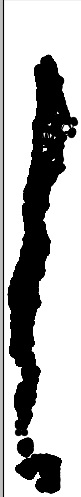
\includegraphics[scale=1]{chile.jpg} 
    %\caption{Descripci\'on si se desea} 
    }
    \centering
\end{figure}
\pagebreak
\label{cap.introduccion}\section{Introducci\'on}

A modo de introducci\'on un archivo \textit{.shp} es un archivo de datos que contiene  lo necesario para obtener la forma de un lugar en el espacio y sus coordenadas. Se obtuvieron los archivos necesarios para el problema de  www.bcn.cl \\
Para abrir este tipo de archivo es necesario instalar el package ''shapefile'', adem\'as, por ser sistema operativo W10 es necesario mantener el archivo .shp en la misma carpeta que el package.
As\'i obtenemos la forma de Chile a nivel comunal, sin embargo lo necesitamos triangularizado, es por esto que con la ayuda del package ''triangle'' obtenemos lo siguiente como muestra.
\begin{figure}[H]
  \scalebox{0.5}{
  
    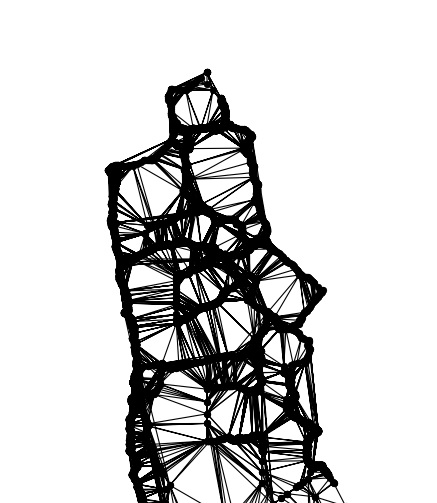
\includegraphics[scale=1]{chile2.jpg} 
    %\caption{Descripci\'on si se desea} 
    }
    \centering
\end{figure}

\label{cap.introduccion}\section{Formulaci\'on Matem\'atica primer m\'etodo}
Se sabe que la ecuaci\'on de centro de masa en su forma general es 

\begin{equation}
I=\dfrac{\int_{\Omega} \overline{x}\rho(\overline{x}) dS(\overline{x}) }{\int_{\Omega} \rho(\overline{x}) dS(\overline{x}) }
\end{equation}
Como el problema se desarrolla a nivel comunal,  sabemos que $\rho(\overline{x})$ es constante por cada comuna. As\'i  desarrollamos la ecuaci\'on $(2.1)$ para cada comuna, luego desarrollamos para cada triangulo de la comuna de la siguiente manera, por separado el numerado y luego el denominador
\begin{equation}
\int_{\Omega} \overline{x}\rho(\overline{x}) dS(\overline{x})=\sum_{comunas} \lbrace \rho_{comunas} \sum_{T_c} \int_{T_c} \overline{x} dS(\overline{x}) \rbrace 
\end{equation}
\begin{equation}
\int_{\Omega} \rho(\overline{x}) dS(\overline{x})=\sum_{comunas} \lbrace \rho_{comunas} \sum_{T_c} \int_{T_c}  dS(\overline{x}) \rbrace 
\end{equation}
Sin embargo nos encontramos con un problema, esto puede resolverse siempre y cuando las coordenas que tenemos en nuestro archivo est\'en en coordenadas cartesianas. Como es de esperar las coordenas del archivo divisi\'on\_ comunal.shp no est\'a en ninguna coordenada cartesiana, es por ello que  usaremos coordenadas esf\'ericas para continuar con la resoluci\'on del problema.\\

A partir de aqu\'i vemos que es necesario cambiar las coordenadas a esf\'ericas, o  m\'as bien a coordenadas geograficas con $(\theta,\phi)$ para ello usamos  el package ''utm'' de python, en el cual es necesario  colocar como entrada la posici\'on de los ejes, la zona y el numero indicador, es decir $19,K$ en este caso.

El cambio de variables es el siguiente
\[\hat{x}=sin(\theta)cos(\phi)\hat{r}+cos(\theta)cos(\phi)\hat{\theta}-sin(\phi)\hat{\phi} \]
\[\hat{y}=sin(\theta)sin(\phi)\hat{r}+cos(\theta)sin(\phi)\hat{\theta}+cos(\phi)\hat{\phi} \]
\[\overline{z}=cos(\theta)\hat{r}-sin(\theta) \hat{\theta}\]
Para simplicidad del ejercicio supondremos que la tierra es una circunferencia, es decir el radio es constante $R=6371000m$. As\'i solo basta resolver las integrales para $(\theta,\phi)$.
Dado un triangulo $T$, la integral sobre ese triangulo quedar\'a de la siguiente manera

\begin{equation}
\int_{\Omega} \overline{x}\rho(\overline{x}) dS(\overline{x})=\sum_{comunas} \lbrace \rho_{comunas} \sum_{T_c} \int_{T_c((\theta,\phi))} \overline{x}(\theta,\phi) R^2 cos(\theta)d\theta d\phi) \rbrace 
\end{equation}
\begin{equation}
\int_{\Omega} \rho(\overline{x}) dS(\overline{x})=\sum_{comunas} \lbrace \rho_{comunas} \sum_{T_c} \int_{T_c((\theta,\phi))} R^2 cos(\theta)d\theta d\phi) \rbrace 
\end{equation}
Como el radio es constante solo nos queda resolver las siguientes integrales para $\theta$ y $\phi$.
Por esto vemos que, dado un triangulo $T(\theta ,\phi)$ delimitado de la siguiente  forma, la primera si formando el lado recto del triangulo rect\'angulo izquierdo, la segunda formando el triangulo rect\'angulo derecho
\[ T+=\lbrace(\phi, \theta) | a \leq \phi \leq b \wedge c \leq \theta \leq d (\phi-a) + c \rbrace\] 
\[ T-=\lbrace(\phi, \theta) | a \leq \phi \leq b \wedge c \leq \theta \leq d (b-\phi)d + c \rbrace\] 
Dividimos el triangulo en dos,  con dos caras paralelas a los ejes, entonce para la componente $\theta$ del resultado
\begin{equation}
I_{T+}\hat{\theta}=\int_{a}^{b}\int_{c}^{d (\phi-a) + c}F_{\theta}(\theta,\phi)d\theta d\phi=\int_{a}^{b}\int_{c}^{d (\phi-a) + c} R^2cos(\theta)\lbrace cos(\theta)cos(\phi) +cos(\theta)sin(\phi)-sin(\theta) \rbrace d\theta d\phi
\end{equation}
Para la componente $\phi$ del resultado
\begin{equation}
I_{T+}\hat{\phi}=\int_{a}^{b}\int_{c}^{d (\phi-a) + c}F_{\phi}(\theta,\phi)d\theta d\phi=\int_{a}^{b}\int_{c}^{d (\phi-a) + c} R^2cos(\theta)\lbrace cos(\theta)cos(\phi) +cos(\theta)sin(\phi)-sin(\theta) \rbrace d\theta d\phi
\end{equation}
De manera an\'aloga se obtiene el resultado para las partes derechas del tri\'angulo, solo que al integrar se cambian los l\'imites de integraci\'on por lo que  corresponden al lado derecho. Sin embargo para integrar esto podr\'iamos ocupar el paquete scipy de python, sin embargo para la terminar de python en W10 este paquete no est\'a soportado a menos que sea con Python 3.2. Al momento de programar todo esto ya se hab\'ia avanzado demasiado con la instalaciones de packages en python 3.5, y los problemas que surgieron debido a esto   iban a tomar m\'as tiempo que  insertar la siguiente soluci\'on.\\
En vez de programar todo para usar el paquete scipy, se us\'o el m\'etodo de simpson anidado para  calcular esta integral, es decir para $I_T\hat{\theta}_+$ se integr\'o por regla de simpson $F_\theta$  y luego al resultado se integr\'o nuevamente por regla de simpson con respecto a $\phi$. 

\[I_{T+}\hat{\theta}=\frac{b-a}{6}\lbrace H_1(a)+4H_1(\frac{a+b}{2}) +H_1(_b) \rbrace\] 
Con $H$ definida  como la integral usando el m\'etodo de simpson
\[H_1(\phi)=\dfrac{\overline{\phi}-c}{6}\lbrace F_{\theta}(c,\phi) +4 F_{\theta}(\frac{c+\overline{\phi}}{2},\phi) +F_{\theta}(\overline{\phi},\phi) \rbrace\]
con
\[\overline{\phi}=(\phi-a)d+c\]
\pagebreak

De manera an\'aloga procedemos para $I_T\hat{\phi}$
\[I_{T+}\hat{\phi}=\frac{b-a}{6}\lbrace H_2(a)+4H_2(\frac{a+b}{2}) +H_2(b) \rbrace\] 
Con $H$ definida  como la integral usando el m\'etodo de simpson
\[H_2(\phi)=\dfrac{\overline{\phi}-c}{6}\lbrace F_{\phi}(c,\phi) +4 F_{\phi}(\frac{c+\overline{\phi}}{2},\phi) +F_{\phi}(\overline{\phi},\phi) \rbrace\]
con
\[\overline{\phi}=(\phi-a)d+c\]
Luego hacemos lo mismo para la parte de la derecha de cada triangulo en cada comuna. Es decir para $I_T\hat{\theta}_-$ y $I_T\hat{\phi}_-$ De esta manera
\begin{equation}
\int_{\Omega} \overline{x}\rho(\overline{x}) dS(\overline{x})=\sum_{comunas} \lbrace \rho_{comunas} \sum_{T_c}  I_{T+}\hat{\theta}+I_{T+}\hat{\phi}+I_{T-}\hat{\theta}+I_{T-}\hat{\phi} \rbrace 
\end{equation}
Siguiendo este razonamiento podemos llegar a una expresi\'on para el denominador.
\begin{equation}
\int_{\Omega} \rho(\overline{x}) dS(\overline{x})=\sum_{comunas} \lbrace \rho_{comunas} \sum_{T_c} IT_c \rbrace 
\end{equation}
con
\begin{equation}
IT_c=\frac{b-a}{6}\lbrace H_3(a)+4H_3(\frac{a+b}{2}) +H_3(b) \rbrace
\end{equation}

\begin{equation}
H_3(\phi)=\frac{\overline{\phi}-c}{6}\lbrace G(c,\phi)+4G(\frac{\overline{\phi}+c}{2},\phi) +G(\overline{\phi},\phi) \rbrace
\end{equation}
\begin{equation}
G(\theta,\phi)=R^2cos(\theta)(cos(\phi)-sin(\phi))
\end{equation}
De esta manera, en teor\'ia deber\'iamos finalmente podemos obtener de manera ''poco precisa'' el centro de masa.
Programar esto en python 3.5 no es sencillo, sin embargo no  imposible.\\
Los archivos que traen la informaci\'on tienen algunos espacios que dificultaron la tarea de programar, se tuvo que asignar la densidad de cada comuna a mano, ya que  los datos estaban ordenados sin un patr\'on en el archivo .shp, adem\'as de las dificultades de compatibilidad entre python y W10 dificultaron demasiado. 
\pagebreak

\label{cap.introduccion}\section{Resultados num\'ericos con este primer m\'etodo}
Usando el procedimiento descrito arriba los resultados  que arroja python son los siguientes.
\[\theta=-7.500589,\phi=-50.841106\]
Es claro que estos resultados no son concluyentes, ni mantienen un significado en la descripci\'on geogr\'afica de Chile, el error podr\'ia deberse a error de tipeo, al traspasar los pesos o  al momento de  generar la integral. Adem\'as en la programaci\'on por compatibilidad de software algunas comunas debieron ser descartadas porque entregaban valores $nan$. \\

Sin embargo otro camino, que no se tom\'o porque la base del archivo shp no era cartesiana,era integral de manera inmediata sin pasar por un cambio de coordenadas, usando la regla de integraci\'on sobre un triangulo de coordenadas $(x_1,y_1),(x_2,y_2),(x_3,y_3)$ donde $|T|$ es el \'area del triangulo
\[I_T=\frac{x_1+x_2+x_3}{3}|T|+\frac{y_1+y_2+y_3}{3}|T|\]
Con este m\'etodo, la programaci\'on se vuelve mucho m\'as sencilla y el programa en python entrega valores m\'as razonables
\[x=311288.1868\]
\[y=6773726.6466\]
Luego transformamos estos datos y nos entregan
\[\theta=-29.1510\]
\[\phi=-70.9401\]
Luego buscamos este punto con la ayuda de Google earth
\begin{figure}[H]
  \scalebox{0.5}{
  
    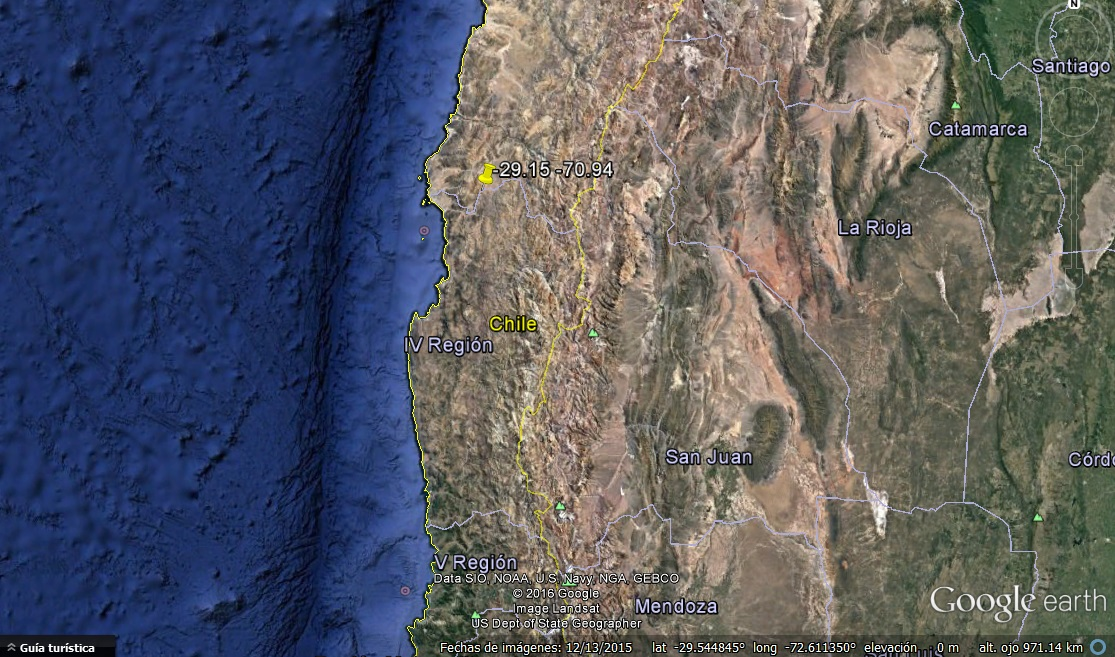
\includegraphics[scale=1]{chile3.jpg} 
    %\caption{Descripci\'on si se desea} 
    }
    \centering
\end{figure}
\label{cap.introduccion}\section{Formulaci\'on Matem\'atica segundo m\'etodo}
Como vimos en el primer m\'etodo era necesario triangularizar  nuestras zonas para poder tener las integrales, este capitulo tratar\'a de resolver  este problema sin usar la triangularizaci\'on. \\
En primer lugar en el programa ser\'a realizado en Python 2.17, y se usar\'an los packages GDAL y Scipy, estos son necesarios para poder tener las coordenadas en  $\phi,\theta$ las cuales  conocemos y podemos usar para resolver las integrales de la siguiente manera.
\\
\\

Sea $D$ una regi\'on de v\'ertices $(\varphi_0, \theta_0)$, $(\varphi_1, \theta_1)$, $(\varphi_2, \theta_2)$,...,$(\varphi_p, \theta_p)$ dados en sentido antihorario; esto es,
\begin{equation}\label{T}
D = \left\{ \sum_{i=0}^p t_i (\varphi_i, \theta_i) \mid 0 \leq t_0, t_1, t_2,...,t_p \leq 1 \ \wedge \ t_0+t_1+t_2+...+t_p=1 \right\}.
\end{equation}
Deseamos computar las integrales

\begin{equation}\label{I1}
I_{D,x} := \int_D x(\varphi, \theta) \rho_D(\varphi,\theta) dS(\varphi, \theta) 
\end{equation}
\begin{equation}\label{I1}
I_{D,y} := \int_D y(\varphi, \theta) \rho_D(\varphi,\theta) dS(\varphi, \theta) 
\end{equation}
\begin{equation}\label{I1}
I_{D,z} := \int_D z(\varphi, \theta) \rho_D(\varphi,\theta) dS(\varphi, \theta) 
\end{equation}
Para evitar calcular directamente estas integrales usaremos el teorema de la divergencia, para ello primero expresaremos cada una de estas integrales en  sus coordenadas $(\varphi, \theta)$
\\
Usando el hecho que:
\[x=R\sin(\theta)\cos(\varphi),y=R\sin(\theta)\sin(\varphi),z=R\cos(\theta) \]
\begin{equation}\label{I1}
I_{D,x} := \int_D  R^2\sin^2(\theta)\cos(\varphi) dS(\varphi, \theta) 
\end{equation}
\begin{equation}\label{I1}
I_{D,y} := \int_D R^2\sin^2(\theta)\sin(\varphi) \rho_D(\varphi,\theta) dS(\varphi, \theta) 
\end{equation}
\begin{equation}\label{I1}
I_{D,z} := \int_D R^2\cos(\theta)\sin(\theta) \rho_D(\varphi,\theta) dS(\varphi, \theta) 
\end{equation}
Para ocupar el teorema de la divergencia primero encontraremos antidiergencia para cada uno de los integrandos anteriores, lo cual no es dificil. Dado que la densidad en cada regi\'on D es constante este termino podemos dejarlo afuera, al igual que el Radio de la tierra R.
\begin{equation}\label{F}
F_x(\varphi, \theta) = \frac{5}{4}\begin{bmatrix}
\cos(\varphi)(-\frac{1}{5}\sin(2\theta))\\[2ex]
\sin(\varphi)(\frac{-1}{2}+\frac{\cos(2\theta)}{10})
\end{bmatrix}
\end{equation}
%
\begin{equation}\label{F}
F_y(\varphi, \theta) = \frac{1}{2}\begin{bmatrix}
-\sin^2(\theta)\cos(\theta) \\[2ex]
\sin(\varphi)(\frac{\theta}{2}-\frac{\sin(2 \theta)}{4})
\end{bmatrix}
\end{equation}
\begin{equation}\label{F}
F_z(\varphi, \theta) = \frac{1}{4}\begin{bmatrix}
0\\[2ex]
-cos(2\theta)
\end{bmatrix}
\end{equation}
satisface
%
\pagebreak

\begin{equation*}
\operatorname{div}(F_x)(\varphi,\theta)
= \frac{\partial F_{x1}(\varphi, \theta)}{\partial \varphi} + \frac{\partial F_{x2}(\varphi, \theta)}{\partial \theta}
= \cos(\varphi) \sen(\theta)^2.
\end{equation*}

\begin{equation*}
\operatorname{div}(F_y)(\varphi,\theta)
= \frac{\partial F_{y1}(\varphi, \theta)}{\partial \varphi} + \frac{\partial F_{y2}(\varphi, \theta)}{\partial \theta}
= \sin(\varphi) \sen(\theta)^2.
\end{equation*}
\begin{equation*}
\operatorname{div}(F_z)(\varphi,\theta)
= \frac{\partial F_{z1}(\varphi, \theta)}{\partial \varphi} + \frac{\partial F_{z2}(\varphi, \theta)}{\partial \theta}
= \sin(\theta)\cos(\theta)
\end{equation*}


\begin{equation}\label{I3}
I_{D,x} = \int_{\partial D} F(\varphi, \theta) \cdot \nu_D(\varphi,\theta) dl(\varphi, \theta)
= \sum_{i=0}^{p-1} \int_{E_i} F(\varphi, \theta) \cdot \nu_D(\varphi,\theta) dl(\varphi, \theta),
\end{equation}
%
Donde $\nu_D$ es el vector unitario exterior normal a $D$ definido sobre $\partial D$, $l$ es la medida lineal sobre $\partial D$ y para cada $i \in \{0, 1, 2,..p-1\}$, $E_i$ es el segmento que une a $(\varphi_i, \theta_i)$ con $(\varphi_{i+1}, \theta_{i+1})$
\begin{equation}\label{Ei}
(\forall\,i\in\{0,1,2,...,p-1\}) \quad E_i = \left\{ (1-s) (\varphi_i, \theta_i) + s (\varphi_{i+1}, \theta_{i+1}) \mid 0 \leq s \leq 1 \right\}.
\end{equation}
%
Ahora, usando la parametrizaci\'on de $E_i$ sugerida por \eqref{Ei}, las \'ultimas integrales en \eqref{I3} se pueden escribir en la forma

\begin{multline}\label{lineIntegrals}
\int_{E_i} F(\varphi, \theta) \cdot \nu_T(\varphi,\theta) d l(\varphi, \theta)\\
= \int_0^1 F\big( (1-s) (\varphi_i, \theta_i) + s (\varphi_{i+1}, \theta_{i+1}) \big) \cdot \left[ \frac{1}{\abs{E_i}} \begin{bmatrix} 0 & 1\\-1 & 0\end{bmatrix} \begin{bmatrix} \varphi_{i+1}-\varphi_i \\ \theta_{i+1} - \theta_i \end{bmatrix} \right] \abs{E_i} d s\\
= \int_0^1 F\big( (1-s) (\varphi_i, \theta_i) + s (\varphi_{i+1}, \theta_{i+1}) \big) \cdot \begin{bmatrix} \theta_{i+1}-\theta_i\\ -(\varphi_{i+1} - \varphi_i) \end{bmatrix} d s.
\end{multline}
 
Haciendo esto para $F_x,F_y,F_z$ logramos programar f\'acilmente en Python una rutina para que haga esto para puntos en el mapeo.
\\
Ahora tenemos que:
\begin{equation}
\int_{\Omega} \overline{x}\rho(\overline{x}) dS(\overline{x})=\sum_{comunas} R^2  \lbrace \rho_{comunas} \sum_{D} I_{D,x} + I_{D,y}+ I_{D,z} \rbrace 
\end{equation}
\begin{equation}
\int_{\Omega} \rho(\overline{x}) dS(\overline{x})=Poblacion \hspace{0.1cm} Chile \rbrace 
\end{equation}
De manera an\'aloga se calculo la densidad para cada  comuna.
\begin{equation}
\rho_{comuna}= PoblacionComuna/ \int_{comuna} dS(\overline{x}) \hspace{0.1cm}  \rbrace 
\end{equation}

\label{cap.introduccion}\section{Resultados num\'ericos con este segundo m\'etodo} 
Programando este m\'etodo en Python 2.17 se lograron los siguientes resultados num\'ericos. \\
\[x=-212720.2802713\]
\[y=2529296.374439\]
\[z=-1700162.152957\]
Los cuales llevamos nuevamente a coordenadas en $(\varphi, \theta)$ por la transformaci\'on que existe para ellos y encontramos que:
\[\varphi=-85.19^\circ \]
\[\theta=-56.185^\circ \]
\begin{figure}[H]
  \scalebox{0.5}{
  
    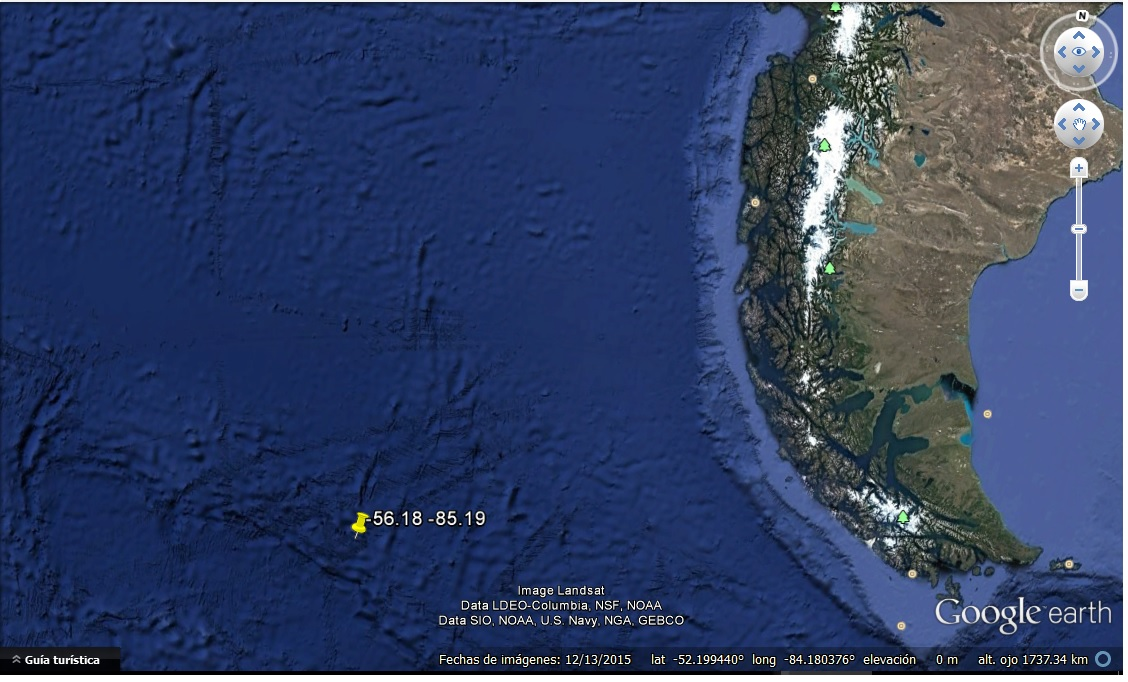
\includegraphics[scale=1]{chile4.jpg} 
    %\caption{Descripci\'on si se desea} 
    }
    \centering
\end{figure}

\section{Conclusiones}
Los resultados num\'ericos para el primer m\'etodo no representan lo que deber\'ian, explicado por alg\'un error en la programaci\'on. Fue necesario acomodar los datos a mano y lo m\'as probable es que se hayan perjudicado en el procedimiento. Sin embargo el camino, la idea de c\'omo llegar a un resultado  m\'as preciso est\'a. El fundamento y la idea de separar cada comuna en  tri\'angulos, para luego integrar sobre ellos es la correcta, tan solo teniendo un buen m\'etodo para conseguir la integral  deber\'ia bastar. Todo esto para la posible continuaci\'on del proyecto en el futuro.\\

La dificultad de este proyecto m\'as all\'a de la parte matem\'atica fue haber programado en un lenguaje en el que no se ten\'ia  experiencia, sin embargo con el tiempo se logr\'o, a pesar de las incontables frustraciones que llegaron a medida que cada paso logrado. Como recomendaci\'on para la continuaci\'on del proyecto,  se sugiere no usar  software incompatible, y de la misma manera tener un m\'etodo m\'as efectivo para le integraci\'on. Se sugiere  poder lograr una triangularizaci\'on que facilite la integraci\'on.\\

Para el segundo m\'etodo  no se us\'o la triangularizaci\'on pues bastaba con tener el pol\'igono cerrado para lograr tener la integral,  hay que notar que los pol\'igonos eran recorridos en sentido horario por lo que  a cada integral en la programaci\'on se le antepuso un signo menos para corregir esto. Tambi\'en  hay que tomar en cuenta que se originaron ciertos  ``agujeros'' dentro de algunos pol\'igonos, generalmente en el sur de Chile donde el car\'acter  oce\'anico de algunos trozos de tierra lograban originarlos, estos agujeros est\'an  orientados de manera contraria que al pol\'igono externo por lo cual no afectaban realmente la integral ya que se cancelaban al momento de sumarlos

\chapter{Bibliografia}
\item http:\textbackslash \textbackslash  www.bcn.cl \textbackslash siit\textbackslash mapas\_ vectoriales\textbackslash index\_ html
\item https:\textbackslash \textbackslash es.wikipedia.org\textbackslash wiki\textbackslash Coordenadas\_ esf\'ericas
\item https:\textbackslash \textbackslash www.python.org\textbackslash
\end{itemize}
\end{document}

